\documentclass[
    landscape,      % landscape or portrait
    paperwidth = 1200mm,
    paperheight = 900mm,
    fontscale = 0.4,
    margin = 1.7cm,
]{baposter}
\definecolor{lightblue}{rgb}{0.145,0.6666,1}
\usepackage{times}
\usepackage{tikz}
\usepackage{floatrow}
\usepackage{hyperref}
\usepackage[utf8]{inputenc}
%
% these are some of my own latex definitions
%

\newcommand{\lzhu}{\underline{L.~Zhu}}
\renewcommand{\topfraction}{.75}

%%%% for manuscript submission
%\newenvironment{annotation}{\bfseries}{\normalfont}
\newenvironment{annotation}{\color{red}}{\color{black}}
%\newcommand{\clearemptydoublepage}{\newpage{\pagestyle{empty}\cleardoublepage}}

%%% for inserting figures
\newcommand{\putfigure}[2]{%
  \begin{center}
%    \epsfig{file=#2,width=#1}
     \includegraphics[width=#1]{#2}%
  \end{center}
}

% two figs left and right aligned at the bottom
\newcommand{\putfigureLR}[4]{%
  \begin{center}
     \begin{tabular}{cc}
     \includegraphics[width=#1]{#2} &
     \includegraphics[width=#3]{#4}
     \end{tabular}
  \end{center}
}

% two figs left and right aligned at the bottom
\newcommand{\putfigurecaptionLR}[6]{%
    \hspace{2em}
    \begin{minipage}{#1}
    %\centering
    \footnotesize
    \textbf{#2}
    \itshape
    #3
    \end{minipage}
    \hspace{1em}
    \begin{minipage}{#4}
    % \centering
    \footnotesize
    \textbf{#5}
    \itshape
    #6
    \end{minipage}

}


% four figs left and right
\newcommand{\putfigureLRLR}[5]{%
  \begin{center}
     \begin{tabular}{cc}
     \includegraphics[width=#1]{#2} &
     \includegraphics[width=#1]{#3} \\
     \includegraphics[width=#1]{#4} &
     \includegraphics[width=#1]{#5}
     \end{tabular}
  \end{center}
}

% two figs left and right aligned at the top
\def\imagetop#1{\vtop{\null\hbox{#1}}}
\newcommand{\putfigureLRt}[4]{%
  \begin{center}
     \begin{tabular}{cc}
     \imagetop{\includegraphics[width=#1]{#2}} &
     \imagetop{\includegraphics[width=#3]{#4}}
     \end{tabular}
  \end{center}
}

% three figs in a row
\newcommand{\putfigureLCR}[6]{%
  \begin{center}
     \begin{tabular}{ccc}
     \includegraphics[width=#1]{#2} &
     \includegraphics[width=#3]{#4} &
     \includegraphics[width=#5]{#6}
     \end{tabular}
  \end{center}
}

% three figs in a row aligned at the top
\newcommand{\putfigureLCRt}[6]{%
  \begin{center}
     \begin{tabular}{ccc}
     \imagetop{\includegraphics[width=#1]{#2}} &
     \imagetop{\includegraphics[width=#3]{#4}} &
     \imagetop{\includegraphics[width=#5]{#6}}
     \end{tabular}
  \end{center}
}

% one left and two in a column at right
\newcommand{\putfigureLRR}[5]{%
  \begin{center}
     \begin{tabular}{cc}
     \includegraphics[width=#1]{#2} &
     \parbox[b]{#3}{\includegraphics[width=#3]{#4}
     \includegraphics[width=#3]{#5}}
     \end{tabular}
  \end{center}
}

% two left in a column and one at right
\newcommand{\putfigureLLR}[5]{%
  \begin{center}
     \begin{tabular}{cc}
     \parbox[b]{#1}{\includegraphics[width=#1]{#2}\\
     \includegraphics[width=#1]{#3}} &
     \includegraphics[width=#4]{#5}
     \end{tabular}
  \end{center}
}

% one fig at left and text in the right
\newcommand{\putfigureL}[4]{%
  \begin{center}
  \parbox{#1}{\includegraphics[width=#1]{#2}}
  \parbox{#3}{#4}
  \end{center}
}

% two figs at left and text in the right
\newcommand{\putfigureLL}[5]{%
  \begin{center}
  \parbox{#1}{\includegraphics[width=#1]{#2}
              \includegraphics[width=#1]{#3}}
  \parbox{#4}{#5}
  \end{center}
}

% two columns of figs
\newcommand{\putfigureLLRR}[6]{%
  \begin{center}
  \parbox{#1}{\includegraphics[width=#1]{#2}
              \includegraphics[width=#1]{#3}}
  \parbox{#4}{\includegraphics[width=#4]{#5}
              \includegraphics[width=#4]{#6}}
  \end{center}
}

%%% two columns texts
\newcommand{\twocol}[4]{%
  \begin{center}
  \parbox[t][][t]{#1}{#2}
  \parbox[t][][t]{#3}{#4}
  \end{center}
}

%%% slide heading
\newcommand{\slideheading}[1]{%
  \begin{center}
    \large\bf
    \shadowbox{#1}%
  \end{center}
  \vspace{1ex minus 1ex}}

%%% some often used units
\newcommand{\kms}{km/s}
\renewcommand{\deg}{$^\circ$}
\newcommand{\Cel}{{\deg}C}

%%% math symbols: e, d (derivative), i (imaginary), T (transpose)
\newcommand{\me}{\mathrm{e}}
\newcommand{\md}{\mathrm{d}}
\newcommand{\mi}{\mathrm{i}}
\newcommand{\mT}{\mathrm{T}}

%%% differential operator
\newcommand{\dif}[2]{\frac{\md #1}{\md #2}}
\newcommand{\ddif}[2]{\frac{\md^2 #1}{\md #2^2}}
\newcommand{\dd}[1]{#1^{\prime\prime}}
\newcommand{\ddd}[1]{#1^{\prime\prime\prime}}
\newcommand{\pdif}[2]{\frac{\partial #1}{\partial #2}}
\newcommand{\pdifc}[2]{{#1}_{,#2}}
\newcommand{\pddif}[2]{\frac{\partial^2 #1}{\partial #2^2}}
\newcommand{\pdddif}[3]{\frac{\partial^2 #1}{\partial #2\partial #3}}
\newcommand{\grad}{\nabla}
\newcommand{\rgrad}{\overrightarrow{\grad}}
\newcommand{\lgrad}{\overleftarrow{\grad}}
\renewcommand{\div}{\nabla\cdot}
\newcommand{\curl}{\grad \times}
\newcommand{\laplace}{\grad^2}
\newcommand{\sgn}{\operatorname{sgn}}

\providecommand{\conjg}[1]{#1^{*}}
\providecommand{\abs}[1]{\lvert#1\rvert}
\providecommand{\norm}[1]{\lVert#1\rVert}

%%%  vectors
\newcommand{\vct}[1]{\mathbf{#1}}
\newcommand{\uct}[1]{\hat{\mathrm{#1}}}

%%% matrices
\newcommand{\mtx}[1]{\mathbf{#1}}

%%% tensors
\newcommand{\tensor}[1]{\mathbf{#1}}

%%% isotopes
\newcommand{\isotope}[2]{{}^{#1}#2}

\def\cossin{\begin{pmatrix}\cos{n \theta}\\ \sin{n \theta}\end{pmatrix}}
\def\sincos{\begin{pmatrix}\sin{n \theta}\\ \cos{n \theta}\end{pmatrix}}

%\DeclareMathOperator\erf{erf}
%\DeclareMathOperator\erfc{erfc}
\endinput


\begin{document}

\begin{poster}{
    % poster environment options
    grid = false,            % true or false
    columns = 3,
    colspacing = 0.6em,
    bgColorOne = white,
    bgColorTwo = white,
    background = plain,     % plain, shade-lr, shade-tb, user, none
    eyecatcher = true,      % eye catcher on the left of the title page
    % posterbox environment options
    borderColor = blue,
    headerColorOne = black,
    headerColorTwo = lightblue,
    headerFontColor = white,
    textborder = roundedleft,   % none, bars, coils, triangles, rectangle
                                % rounded, faded, roundedsmall, roundedleft
                                % roundedright
    headerborder = closed,      % none, closed, open
    headershape = roundedright, % rectangle, small-rounded, roundedleft,
                                % roundedright, rounded
    headershade = shadelr,      % plain, shadelr, shadetb, shade-tb-inverse
    boxshade = none,            % plain, shade-lr, shade-tb, none
    headerfont = \Large\bf\textsc,
    linewidth = 0.1 em,}
{\includegraphics[height=9em]{USTC_logo_blue.jpg}}
{\Huge{3D Crust and Uppermost Mantle Structure beneath Tian Shan Region from Ambient Noise and Earthquake Surface Waves}}
{
    \vspace{0.3em}
    Xiao Xiao$^1$ (\textcolor{blue}{xiaox17@mail.ustc.edu.cn}),
    Lianxing Wen$^{2,1}$ \\
    \vspace{0.3em}
    1. Laboratory of Seismology and Physics of Earth's Interior; School of Earth and Space Sciences, University of Science and Technology of China  \\
    2. Department of Geosciences, Stony Brook University  \\
}
{\includegraphics[height=9em]{Righthand}}
\vspace{0.4cm}

\begin{posterbox}[column=0, row=0]{1. Introduction}
\setlength{\parskip}{3pt}
As a typical active intracontinental mountain range in Central Asia, Tian
Shan Mt. serves as the prototype in studying geodynamic processes and mechanism
of intracontinental mountain building (Fig. 1). Under Tian Shan Mt. and nearby area,
there are three main geological blocks, named as Tarim basin, Tian Shan Mt.
and Junggar basin. To figure out underground structure and geological evolution history there,
we study 3D crust and uppermost mantle structure beneath Tian Shan Mt. and adjoin region
using joint surface wave tomography method based on ambient noise and teleseismic records.
\end{posterbox}

\begin{posterbox}[column=0, below=auto]{2. Data and Method}
\setlength{\parskip}{3pt}
My dataset contains records from 60 brand-band seismic stations, mainly
locating at foot of Tian Shan Mt. and adjoin area (Fig. 1).
Several stations, situating at the sounthern foot of Altai Mt. and northern foot of Kunlun Mt.,
provide critical ray path coverage of Junggar amd Tarim basins. Our dataset includes continuous records
of vertical components from 2015 to 2016 and teleseismic waveforms from 2013 to 2016.
Magnitudes of these earthquakes are over 5.5 and their focal depths are shallower than 200 km.

We combine the group velocity dispersion curves measured from empirical green's functions (EGFs) and teleseismic surface waves,
obtain lateral isotropic Rayleigh group velocity maps at different periods based on traditional surface wave tomography method
and  construct a 3D $V_{sv}$ model down to about 70 km using Markov Chain Monte Carlo method (MCMC).



\begin{center}

\begin{minipage}{0.2\textwidth}
\footnotesize
\textbf{Fig. 1.}
\itshape
Map of study area. Red triangles represent broad-band seismic stations
used in this study. Black lines show the faults.
The insert (top left) depicts telsesimic distribution, in which red circles represent
teleseismic epicenters.
Dashed red rectangle shows the study area. Two red triangles represent two stations
named as AKS and KOL, which are collineation with star-labelled earthquake.
\end{minipage}
\begin{minipage}{0.75\textwidth}
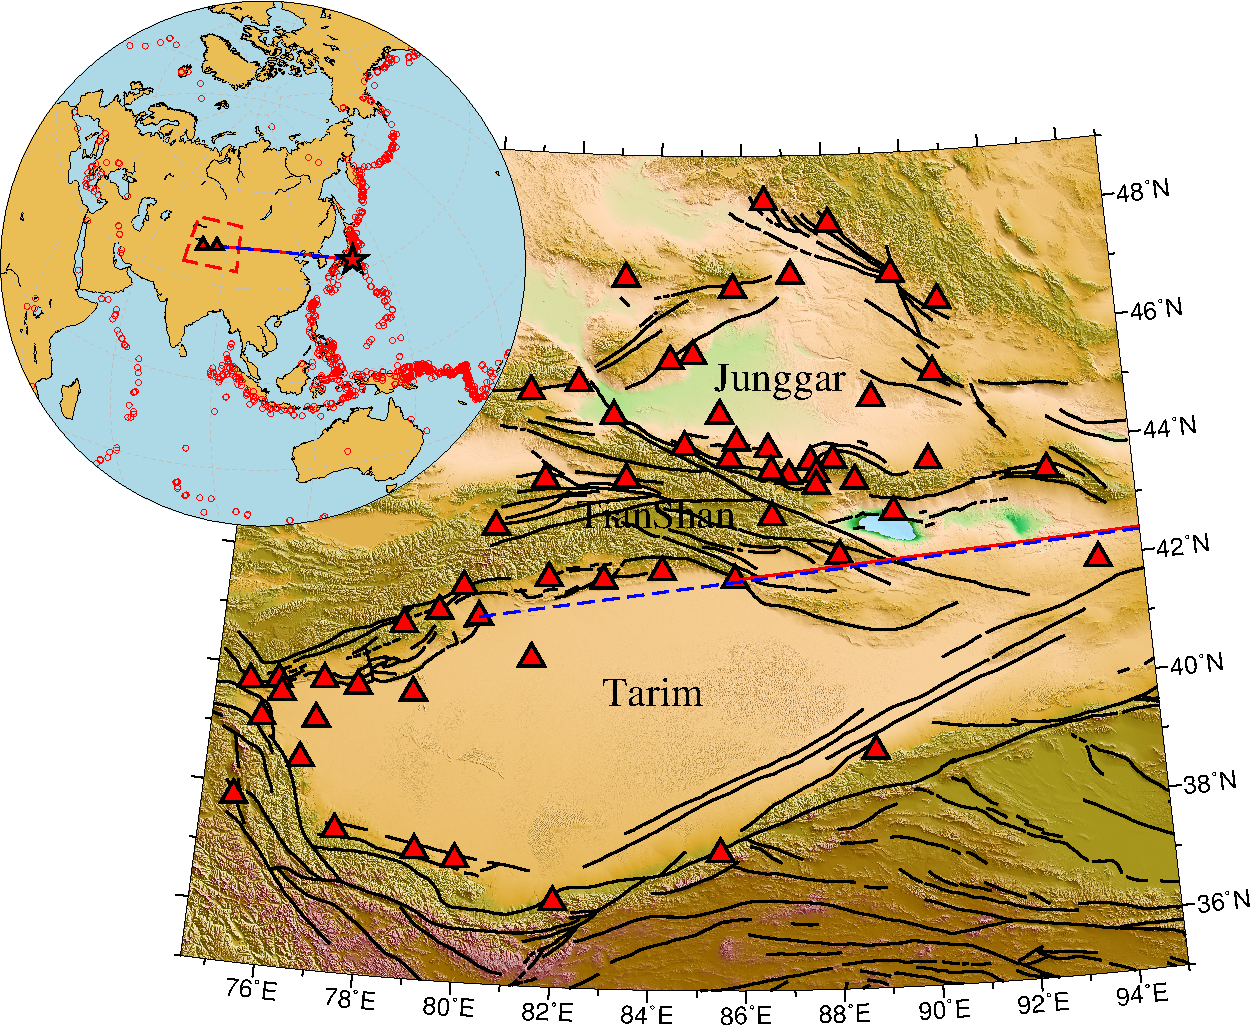
\includegraphics[width=\textwidth]{XJ}
\end{minipage}
\hspace{0.1cm}

\end{center}

We control qualities of dispersion curves with spectral signal-noise-ratio (SNR) and standard deviation of measurements (Fig. 2).
For EGFs, we define signal-noise-ratio (SNR) as ratio of peak in surface wave signal window and root mean standard (rms) in noise window at each period and we measure dispersion curves every trimesters
, which provide standard deviation of dispersion curve between a pair of stations.
We measure dispersion curves from telesemic waveforms of different events with two-station method.
These curves give final dispersion curve with their medians and standard deviations at each periods .

We take averages of reliable dispersion curves, measured from EGFs and teleseismic waveforms to be final
usable dispersion curves (Fig. 3) which are weighted by inverses of their standard deviations. The standard
deviations of final dispersion curves are the summation of those constituents.

\putfigureLR{0.45\textwidth}{Pathnum}{0.45\textwidth}{JointDisp}
\hspace{0.15cm}

\putfigurecaptionLR{0.45\textwidth}
{Fig. 2.}
{Number variation of dispersion curves used for tomography due to dispersion curves quality control. The dashed limegreen line and corresponding limegreen area show
number of used dispersion curves measured from teleseismic waveforms with two-station method while dashed red line and area denote number of those measured from EGFs at each period. The
solid blue line indicates number of all dispersion curves which are summation of above two.}
{0.45\textwidth}{Fig. 3.}
{Demo of group velocity dispersion curve combination between two stations, AKS and KOL.
Red circles denote dispersion points measured from EGF while blue circles represent those estimated from teleseismic waveforms.
Limegreen squares give combined dispersion curve. At overlap periods, green squares are weighted averages of blue and red circles
, in which weights are inverses of their observational error and summation of their errors gives measurement error of combined dispersion curve.
}



\end{posterbox}

\begin{posterbox}[column=1]{3. 2D Group velocity Maps}

With combined dispersion curves, we use traditional surface wave tomography method
to image 2D Rayleigh group velocity maps.

Resolutions shown by fitted radius are
consistent with those shown in checkerboard tests, indicating we can
resolve $222 \ \textit{km} \times 222 \ \textit{km}$ anomalies at Junggar basin,
middle Tian Shan Mt. and  western Tarim basin. However, at the main part of Tarim basin ,
eastern and western parts of Tian Shan Mt., we can only resolve $555 \ \textit{km} \times 555 \ \textit{km}$
anomalies (Fig. 4).

2D Rayleigh group velocity perturbation maps partly show differences between three main geological
blocks. At short periods (10, 26 and 33 s),  perturbation maps are influenced by sedimentary layer, showing
low group velocities in Junggar and Tarim basins. Long period map shows high velocities there, as they are cratons (Fig. 5).

\begin{center}
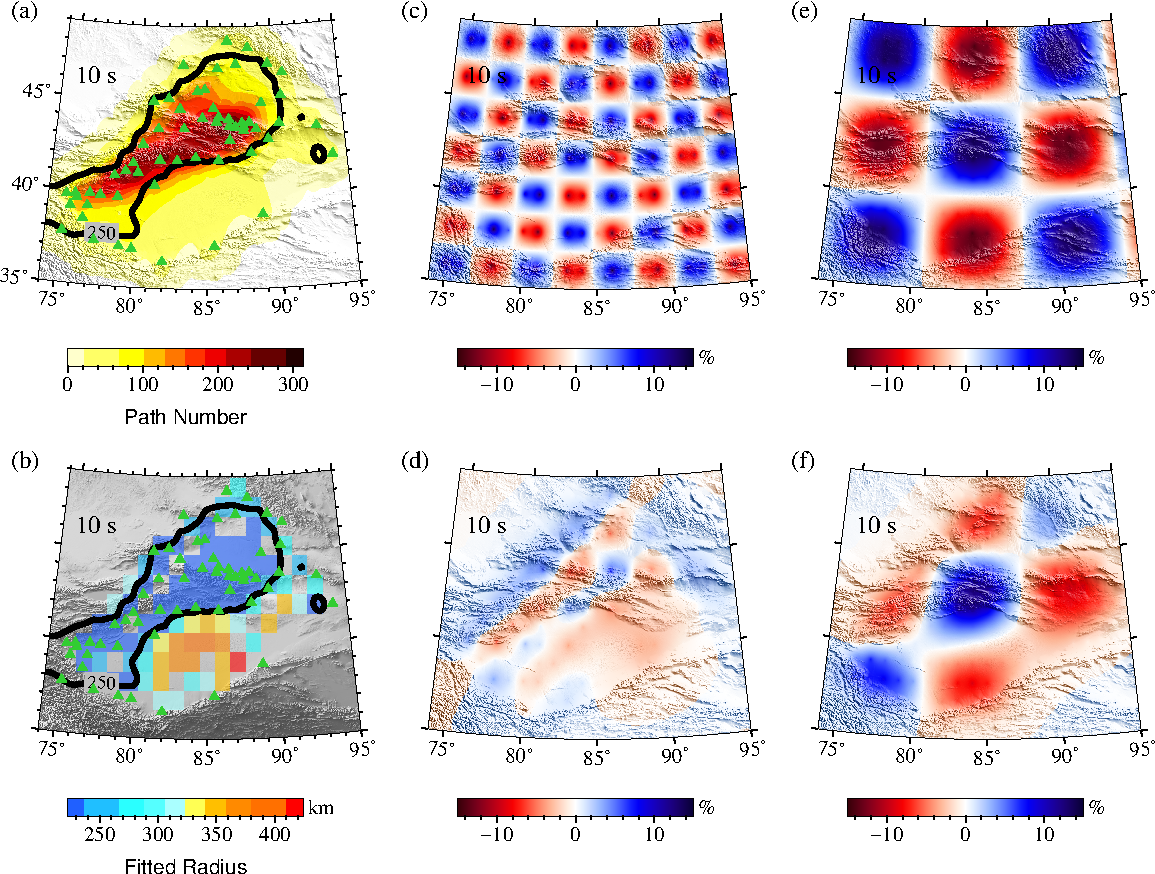
\includegraphics[width=0.75\textwidth]{resolution}
\begin{minipage}{0.9\textwidth}
\footnotesize
\vspace{0.2em}
\textbf{Fig. 4.}
\itshape
Resolution analysis for Rayleigh group velocity tomography at 10 s. (a) Distribution
of path density, indicating path numbers crossing each $1^{\circ} \times 1^{\circ}$ cells.
(b) Distribution of radius, which are fitted from resolution matrix.  In panel (a) and (b),
solid black line encloses area with resolution better than $250$ km.  Limegreen triangles
indicate locations of seismic stations. Panels (c), (d) , (e) and (f) show inputs and outputs of checkerboard tests.
They show Rayleigh group velocity perturbation maps, refering to $2.69315$ km/s which is estimated average group velocity
of study area at 10 s and the colorbars indicate percent of perturbation.
Synthetic model (c) with $222 \ \textit{km} \times 222 \ \textit{km}$ anomalies for checkerboard test and its recovered model (d).
Increasing scale of anomalies up to $555 \ \textit{km} \times 555 \ \textit{km}$, we obtain synthetic model (e) and
recovered one (f).
\end{minipage}
\end{center}

\begin{center}
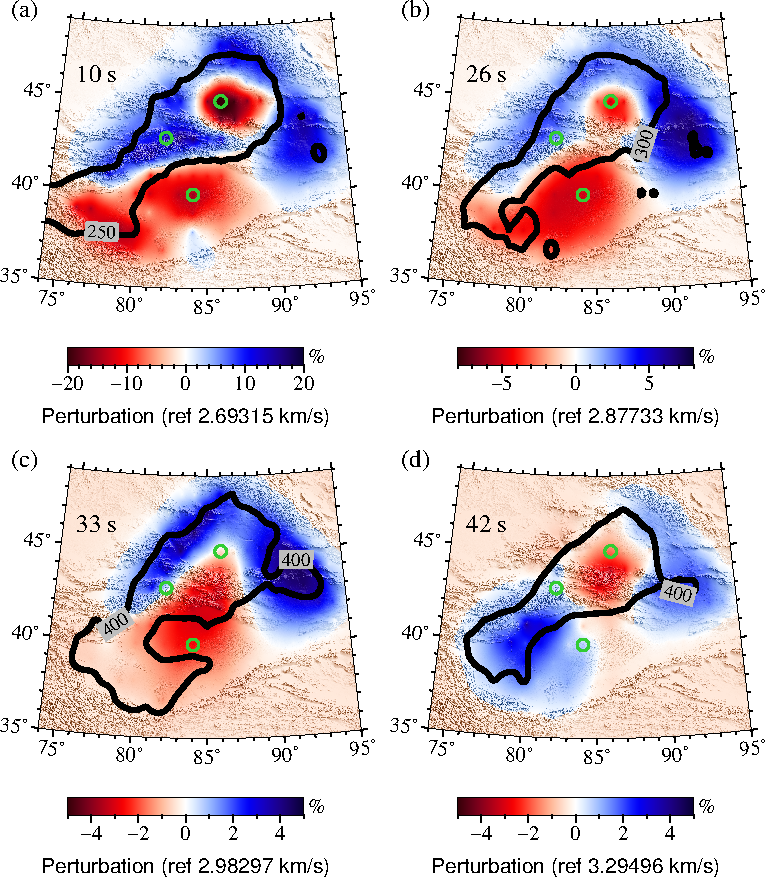
\includegraphics[width=0.75\textwidth]{maps}
\begin{minipage}{0.9\textwidth}
\footnotesize
\vspace{0.2em}
\textbf{Fig. 5.}
\itshape
Rayleigh group velocity perturbation maps at periods
10, 26, 33 and 42 s. The colorbars indicate percent of perturbation, refering to the velocities
denoted in round brackets, which are averages of Rayleigh group velocities in study area at each periods, written
at topleft of each panel. The solid black lines encloses main area with resolution better than
annotated values. Three circles represent representative points of Tarim basin, Tian Shan Mt.
and Junggar basin, separately, where 1D shear velocity models are inverted later.
\end{minipage}
\end{center}

\end{posterbox}

\begin{posterbox}[column=2 ]{4. Shear wave velocity models}
We invert 1D shear velocity model at each points with Markov Chain Monte
Carlo (MCMC) method, based on dispersion curves extracted from above 2D group velocity
maps (Goutorbe, 2015).

\vspace{-0.1cm}
\begin{center}
\begin{tikzpicture}[nodes={inner sep=0}]
\node (a) at (-0.75,-0.2) {\includegraphics[width=0.33\textwidth]{Tarim}};
\node (b) at (4.2,-0.2) {\includegraphics[width=0.33\textwidth]{tianshan}};
\node (c) at (9.0,-0.2) {\includegraphics[width=0.33\textwidth]{Junggar}};
\node at (-3.05, 3.2) {(a)};
\node at (1.9, 3.2) {(b)};
\node at (6.7, 3.2) {(c)};
\end{tikzpicture}


\begin{minipage}{0.9\textwidth}
\small
\textbf{Fig. 6.}
\itshape
Inverted 1D models at three representative points, locating at Tarim basin, Tian Shan Mt. and Junggar basin, separately.
Observed dispersion curves (solid black lines with error bars) are extracted from previous 2D Rayleigh group velocity maps.
Shade areas show the 95 percent confidence interval of the shear velocity models (below) and corresponding theoretical
group velocity dispersion curves (upper). Red lines depict representative shear velocity models (below)
and their synthetic dispersion curves (upper), which are cloesest to the average of all randomly sampled models at each point.
\end{minipage}
\end{center}

\begin{center}
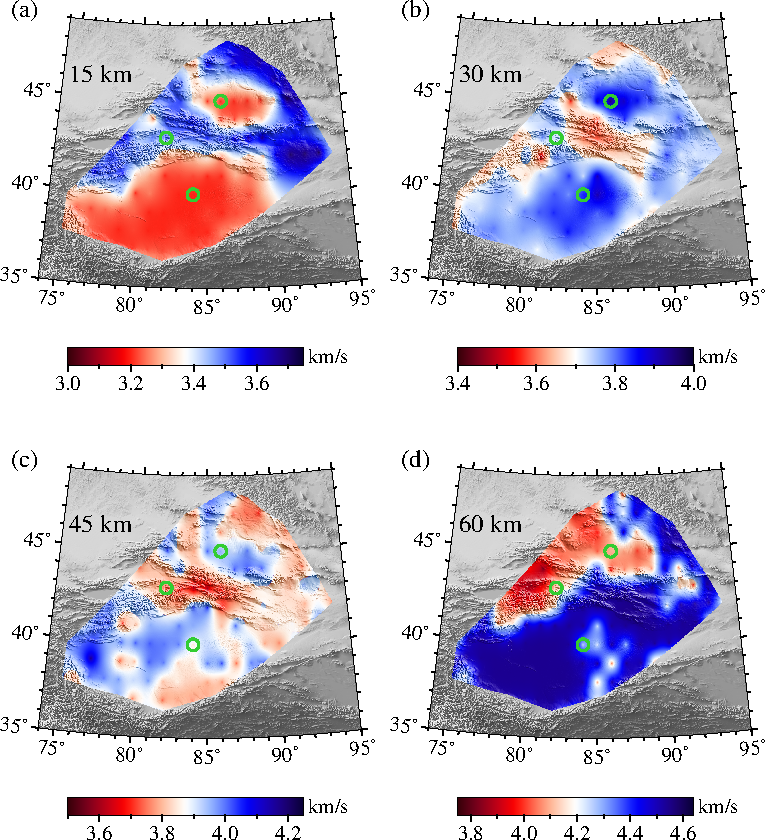
\includegraphics[width=0.75\textwidth]{shear_velocity_maps}
\begin{minipage}{0.9\textwidth}
\footnotesize
\vspace{0.2em}
\textbf{Fig. 7.}
\itshape
 Shear wave velocity maps at depths 15 , 30, 45 and 60 km. The green circles show locations of previous representative 1D shear wave velocity models.
 Study area is divieded to path covered part (colorful area) and that without coverage (dark gray area).

\end{minipage}
\end{center}

\end{posterbox}

\begin{posterbox}[column=2, below=auto]{5. Conclusions}
Current model has multiple resolutions at diffferent regions. It has
$222 \ \textit{km} \times 222 \ \textit{km}$, or even better resolution at
Tian Shan Mt. and Junggar basin and around $555 \ \textit{km} \times 555 \ \textit{km}$ resolution
due to sparseness and nonuniform data coverage at the main part of Tarim basin.

However, it does reflect difference between Tarim, Junggar basins and Tian Shan Mt..
The Tarim and Junggar basins correspond to low shear velocity in upper crust due to sedimentation and
Tian Shan Mt. has high velocity. Things take on the opposite side in middle and lower crust due to the
existence of cratons.
\end{posterbox}

\begin{posterbox}[column=2, below=auto]{6. References}
Goutorbe, Bruno, Diogo Luiz de Oliveira Coelho, and Stéphane Drouet. "Rayleigh wave group velocities at periods of 6–23 s across Brazil from ambient noise tomography." {\itshape Geophysical Journal International} 203.2 (2015): 869-882.
\end{posterbox}

\end{poster}
\end{document}
